%/*% pdflatex -file-line-error -interaction nonstopmode %

\documentclass{article}
\usepackage{graphicx}
\graphicspath{ {./images/} }
\usepackage{amsmath}
\usepackage{amsfonts}
\usepackage{hyperref}
\usepackage{exercises}
\usepackage{amsthm}
\usepackage{yhmath}
\newcommand*{\oldneg}{\mathord{\sim}}

\theoremstyle{definition}
\newtheorem{definition}{Definition}

\setlength{\parindent}{.5in}
\setlength{\parskip}{12pt}

\title{Quiz Exercises}
\begin{document}
\maketitle

\section*{1}
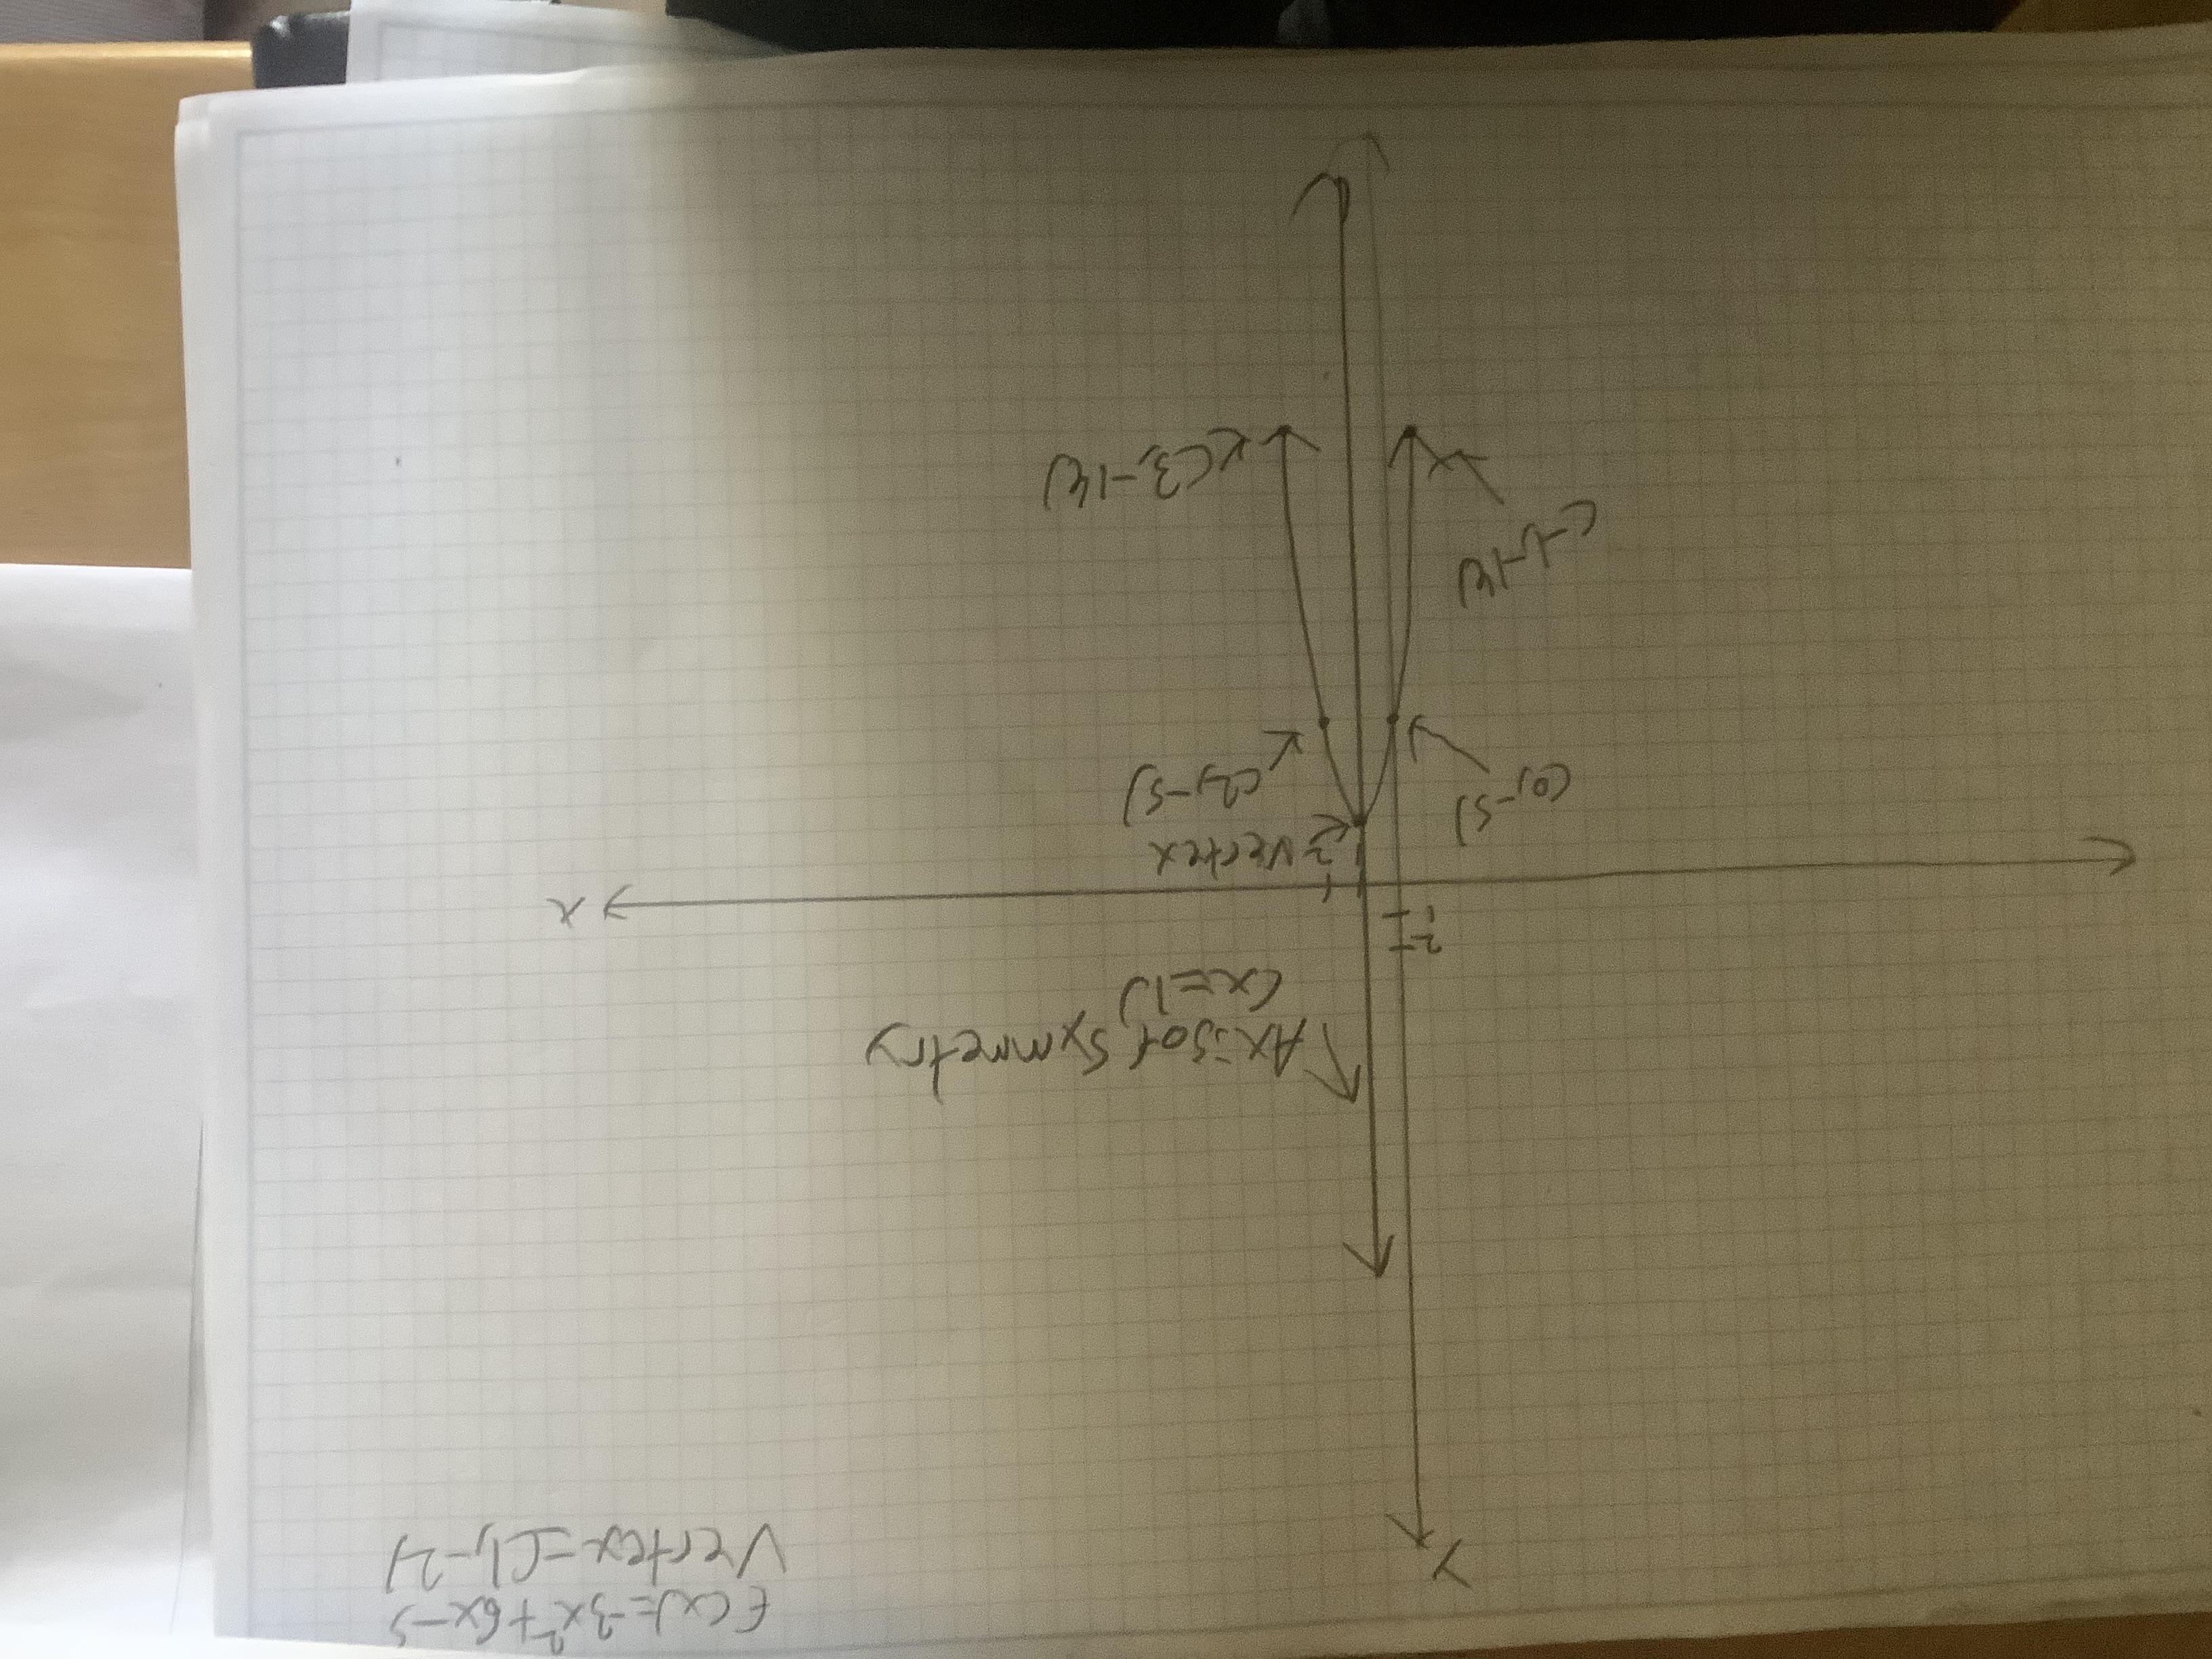
\includegraphics[width = 6in, height = 6in, angle = 180]{picture1}

\section*{2}
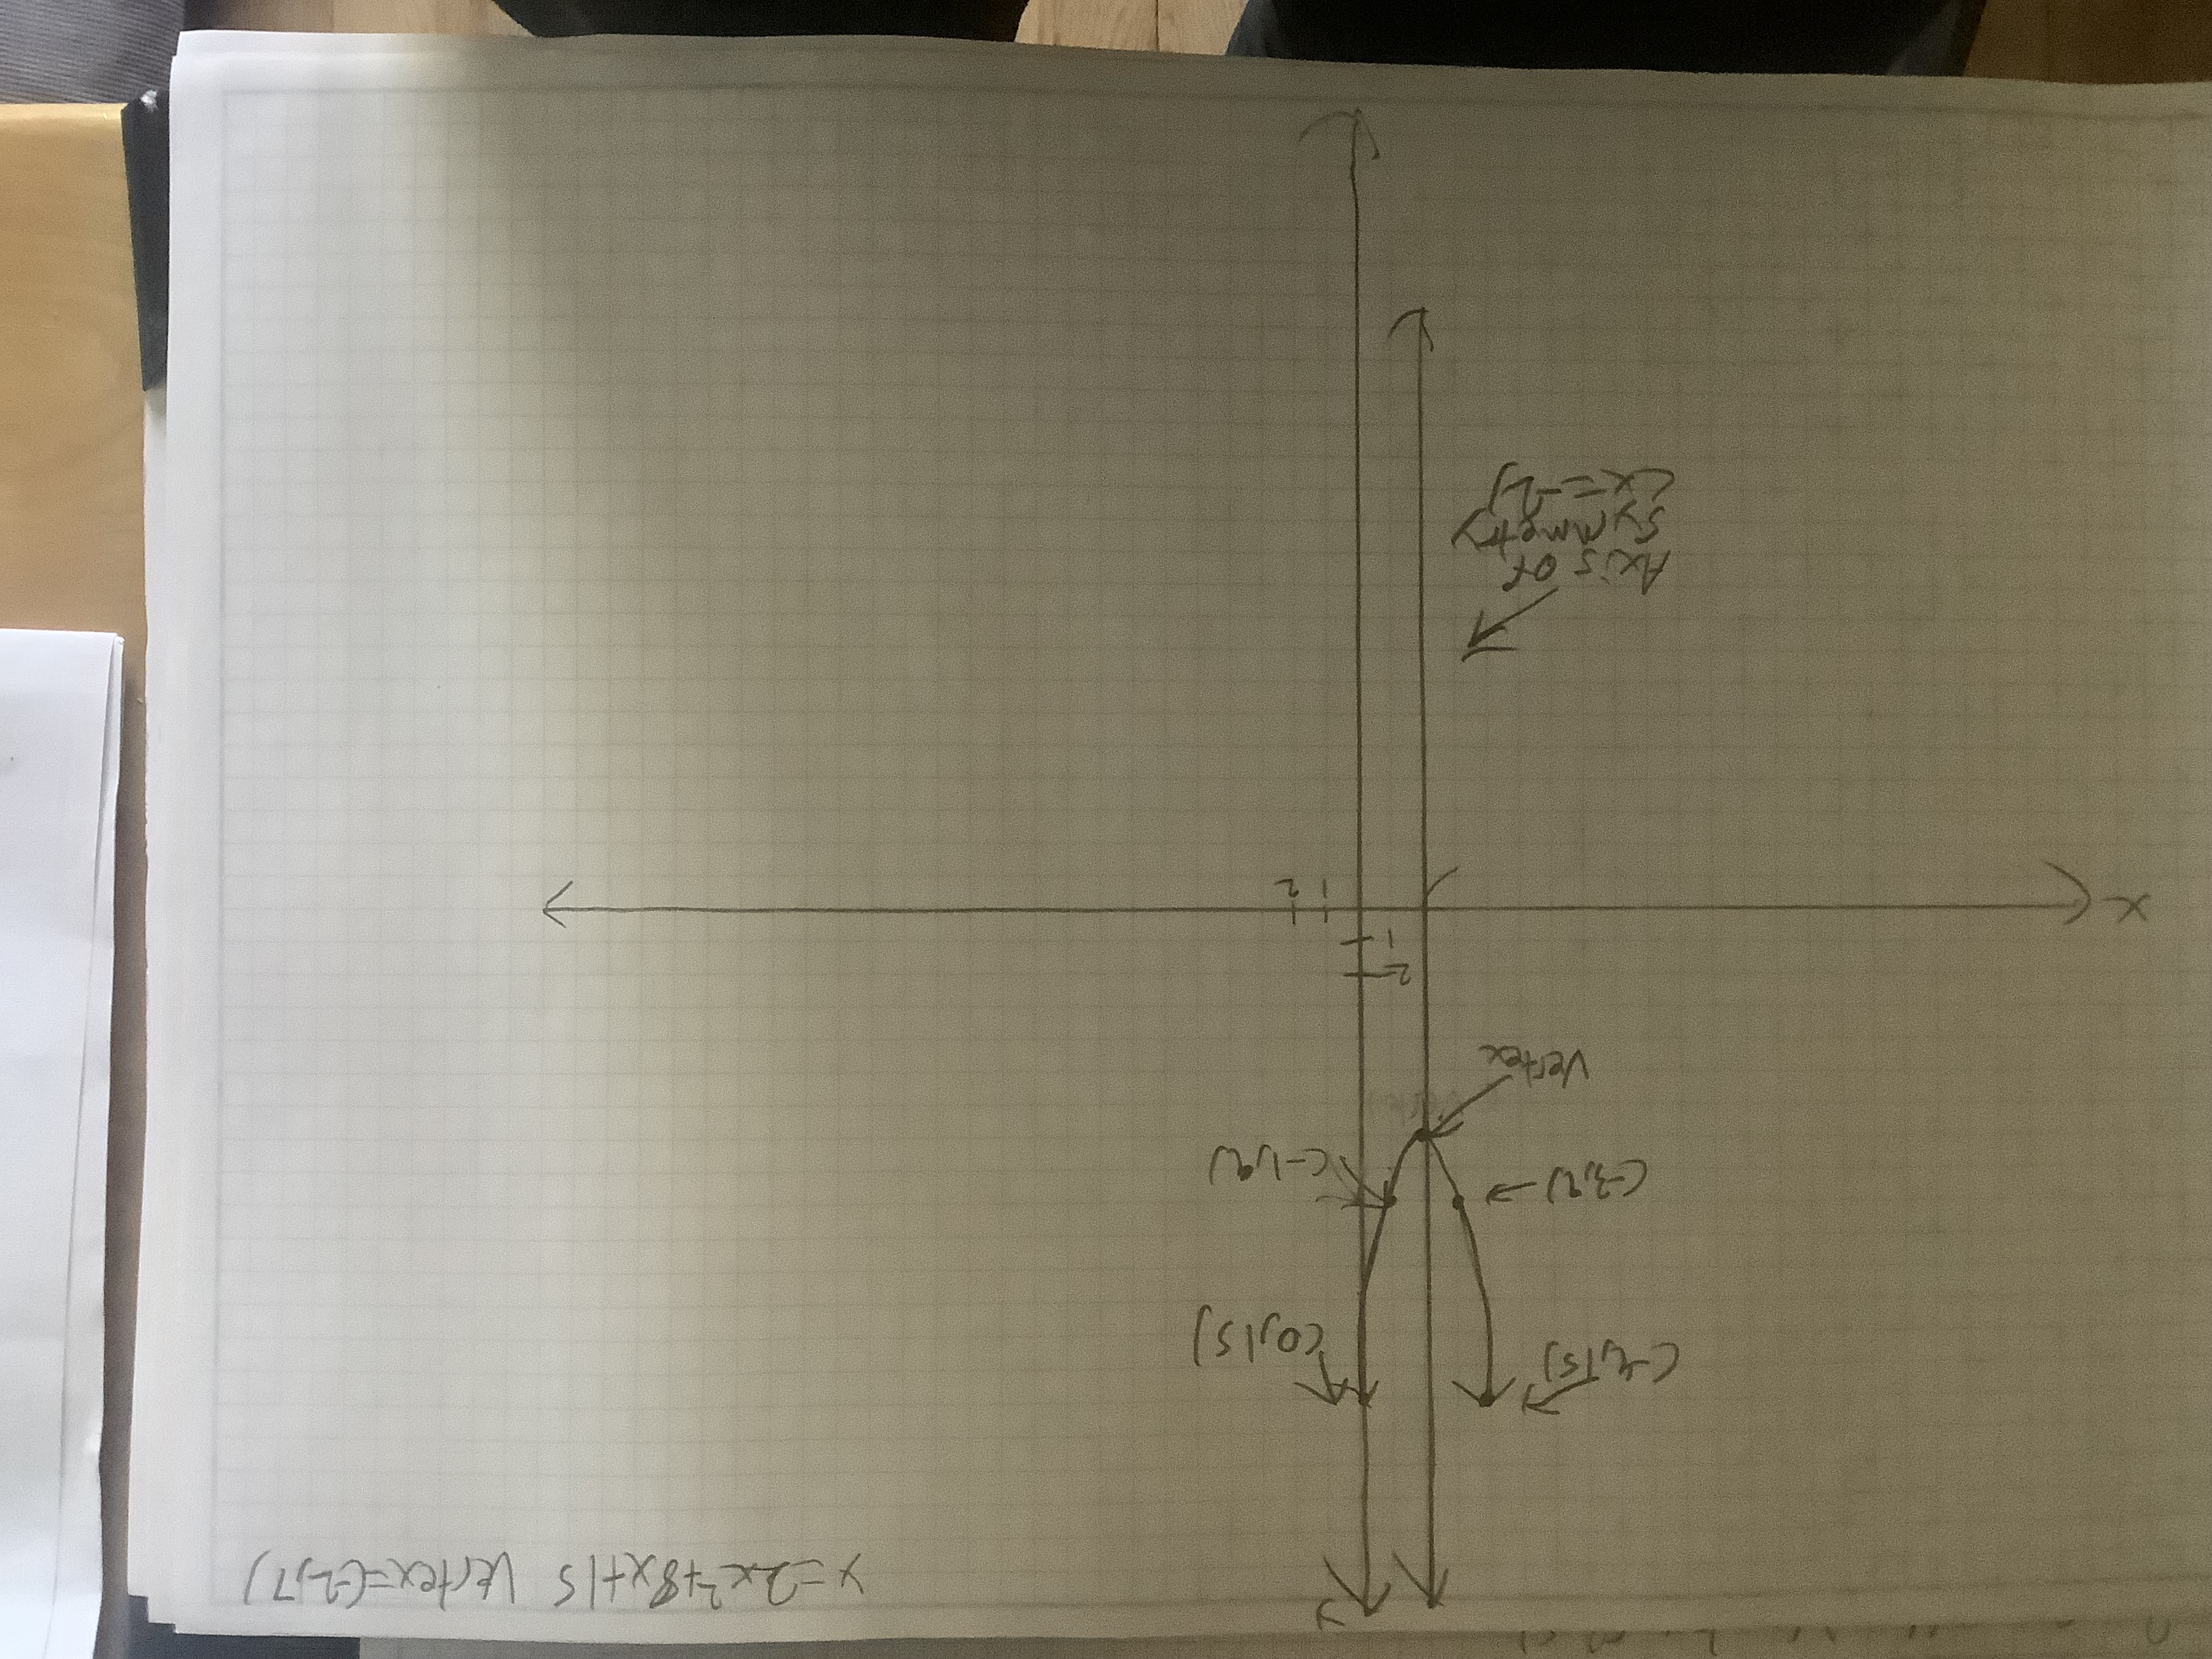
\includegraphics[width = 6in, height = 6in, angle = 180]{picture2}

\section*{3}
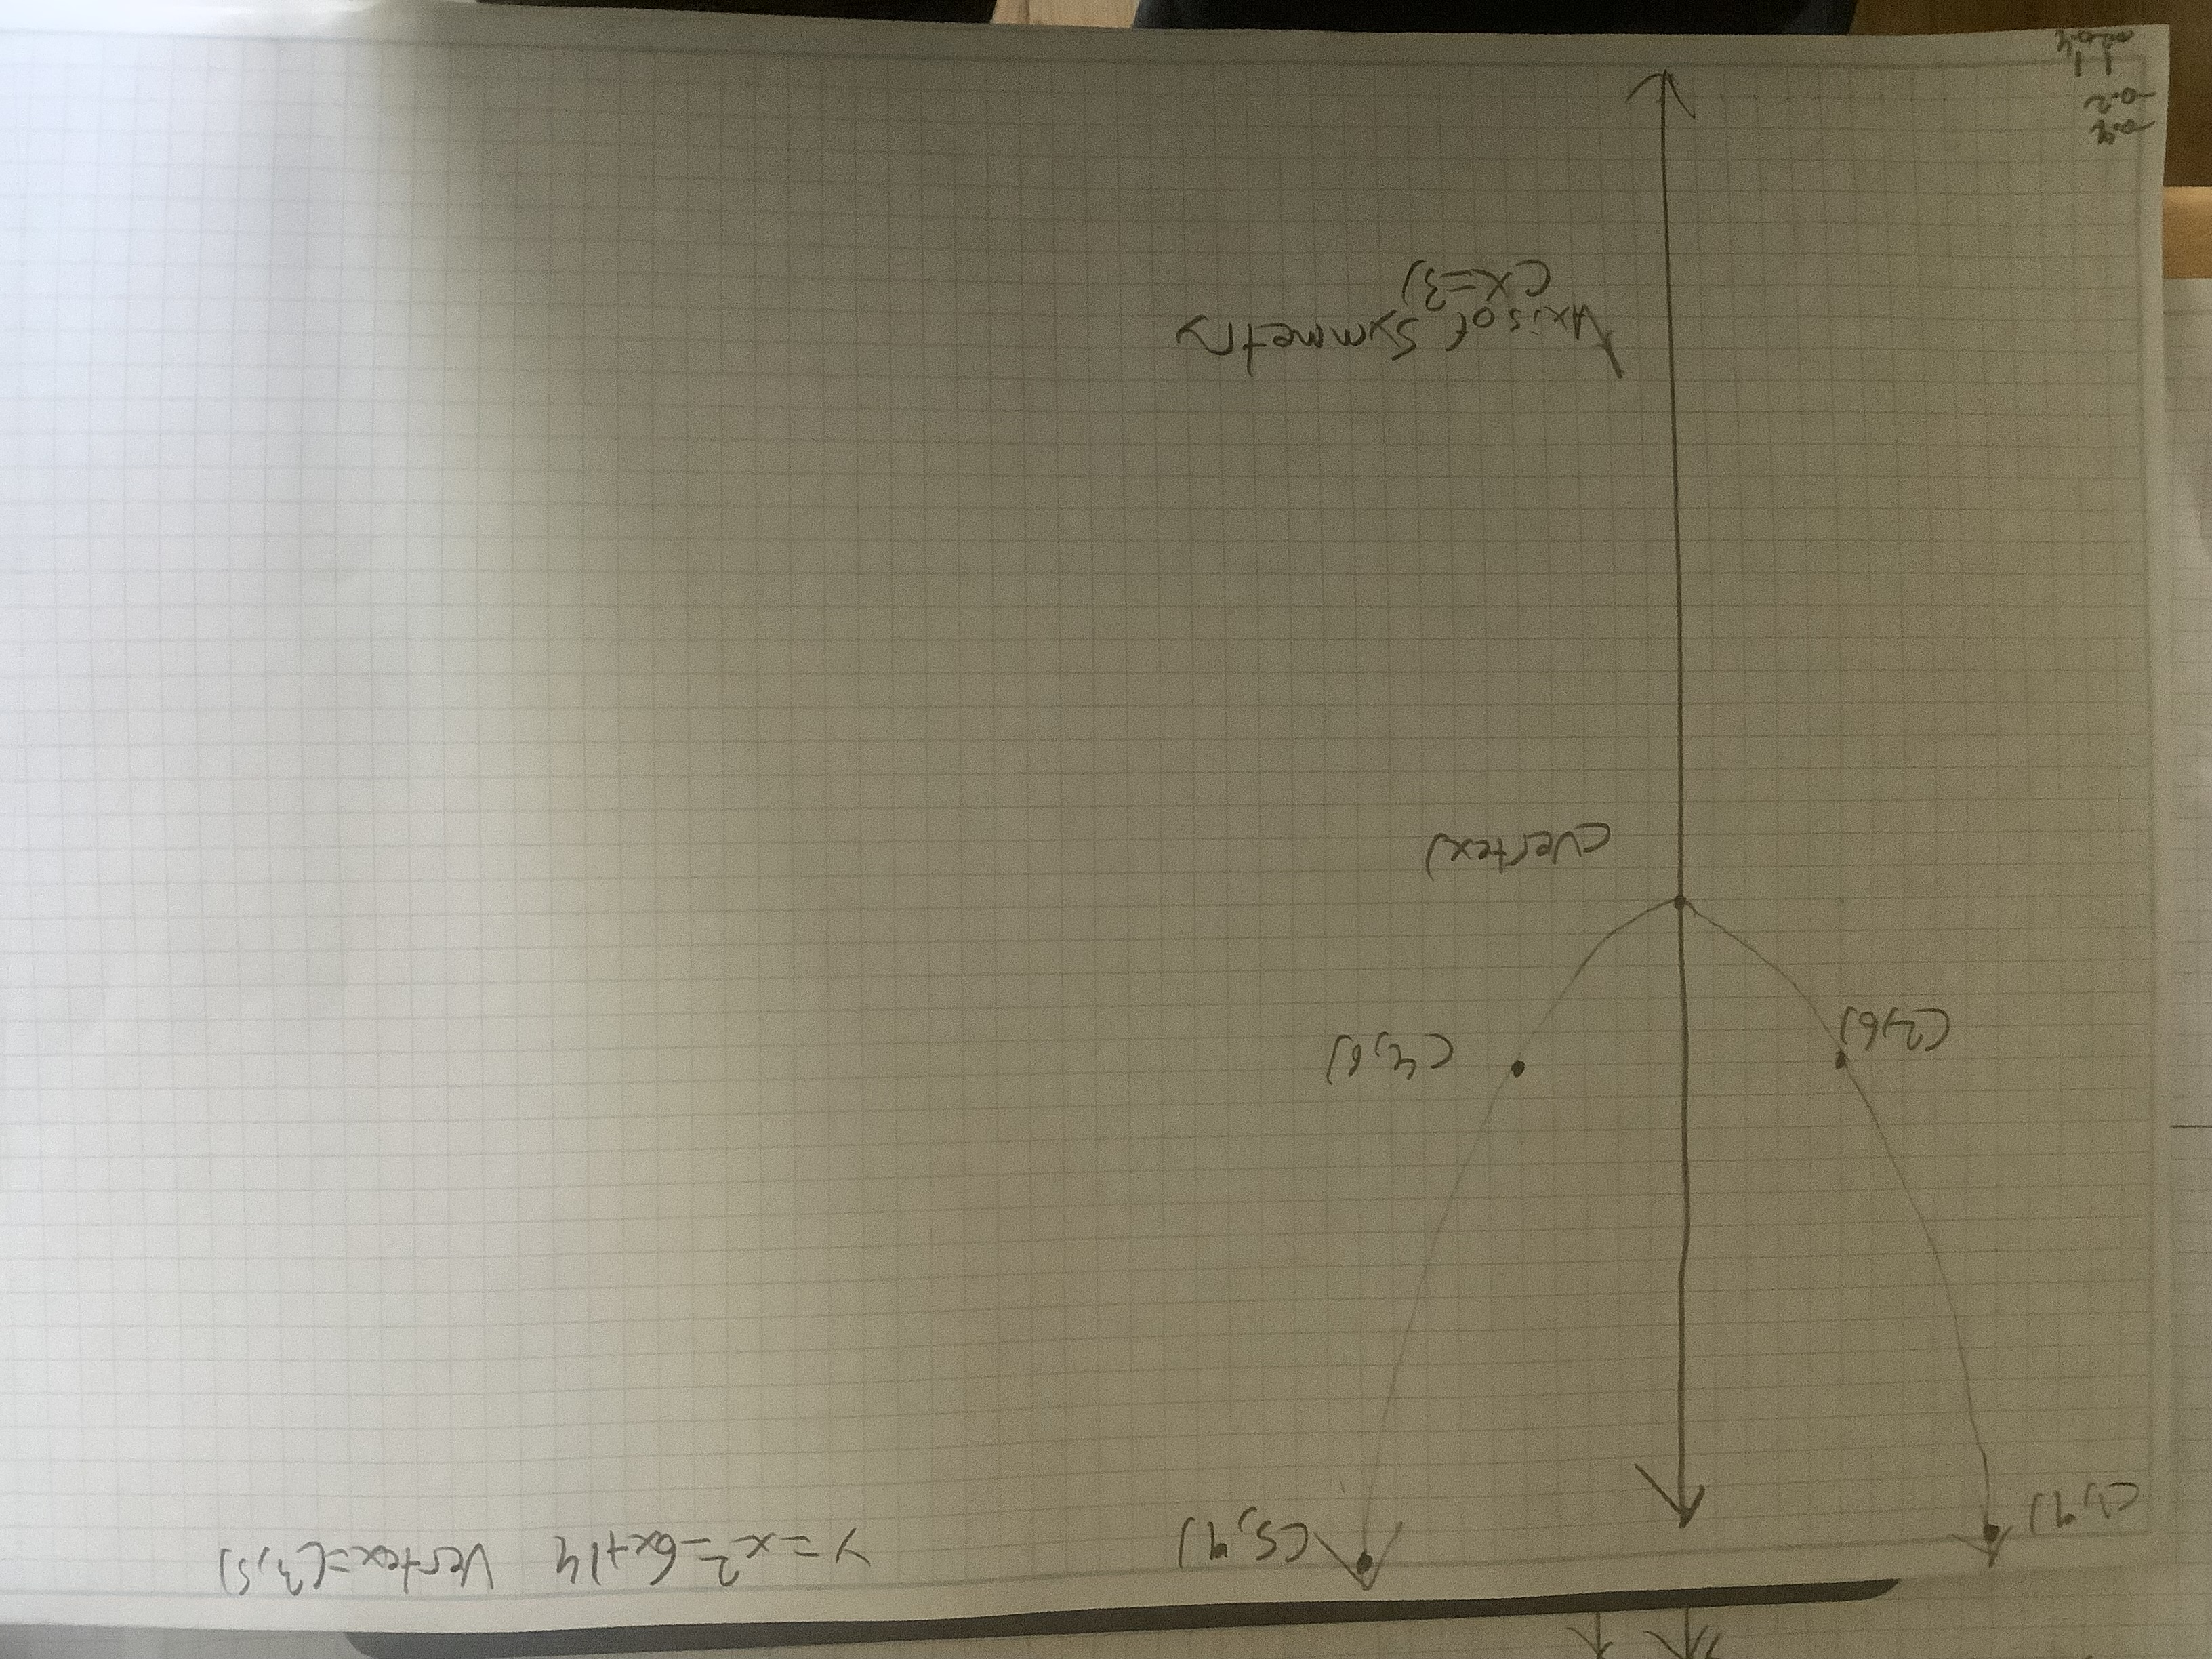
\includegraphics[width = 6in, height = 6in, angle = 180]{picture3}

\section*{4}
$y=(x-4)(x-8)\newline\rightarrow =x^2-12x+32$

\section*{5}
$g(x)=-2(x+3)(x-7)\newline\rightarrow =-2(x^2-4x-21)\newline\rightarrow =-2x^2+8x+42$

\section*{6}
$y=5(x+6)^2-2\newline\rightarrow =5(x^2+12x+36)-2\newline\rightarrow =5x^2+60x+180-2\newline\rightarrow =5x^2+60x+178$

\section*{7}
$x^2+9x+20=0\newline\rightarrow (x+5)(x+4)=0\newline\rightarrow x=-5\vee x=-4$

\section*{8}
$n^2-11n+24=0\newline\rightarrow (n-8)(n-3)=0\newline\rightarrow n=8\vee n=3$

\section*{9}
$z^2-3z-40=0\newline\rightarrow (z-8)(z+5)=0\newline\rightarrow z=8\vee z=-5$

\section*{10}
$5s^2-14s-3=0\newline\rightarrow (5s+1)(s-3)=0\newline\rightarrow s=-\frac{1}{5}\vee s=3$

\section*{11}
$7a^2-30a+8=0\newline\rightarrow (7a-2)(a-4)=0\newline\rightarrow a=\frac{2}{7}\vee a=4$

\section*{12}
$4x^2+20x+25=0\newline\rightarrow (2x)^2+20x+5^2=0\newline\rightarrow (2x+5)^2=0\newline\rightarrow x=-\frac{5}{2}$

\section*{13}
$R(x)=(140-10x)(50+5x)$ First, we find the $x$-coordinate of the vertex, by changing this equation into intercept form:\newline
$-50(x-14)(x+10)$, and thus, the $x$ coordinate is $\frac{14-10}{2}=2$, meaning the maximum value is $(140-10(2))(50+5(2))=7200$. Hence, 
the store should charge $140-10(2)=\$120$ in order to make a maximum profit of $\$7200$.
\end{document}
